\documentclass[english, 12pt, a4paper]{article}
\usepackage[utf8]{inputenc} 
\usepackage[T1]{fontenc,url} %url
\urlstyle{sf} %sf
\usepackage[toc,page]{appendix}
\usepackage{babel,textcomp,csquotes,ifikompendiumforside, varioref,graphicx, gensymb}
\usepackage[]{circuitikz}
\usepackage{tikz}
\usetikzlibrary{shapes,arrows}
\usepackage[backend=biber,style=numeric-comp, sortcites]{biblatex} 
\usepackage{pgfplots}

\bibliography{ref.bib}

% --------------------------------------------------
\title{ \huge{Successive Approximation Register Analog-to-Digital Converter}}
% \subtitle{Legg til en subtitle dersom det trengs}
\author{By Espen Klein Nilsen\\ and Vegard Midtbøen}
% --------------------------------------------------

 


\begin{document}
\ififorside{}
% \frontmatter{}
\maketitle{} \newpage

\tableofcontents{} \newpage
\listoffigures{} 
\listoftables{} \newpage


%-----------Introduksjon-----
% \mainmatter{}        

\section{Introduction} 
Successive Approximation Register (SAR) Analog-to-Digital Converter (ADC) is a common arctitecture whent talking about Analog-to-Digital (A/D) conversion. A/D conversion is used in almost every
circuits today, and the purpose is to convert a signal from the analig to the digital domain. This is of great interest, because digital signals propagates more efficiently than analog singlals in a 
circuit. By using digital signals, it is easier for the electronic circuit to distinguish the signal from the noise \cite{basic-adc}.\\
\\
This task, is as mentrioned, to design a SAR ADC. A block diagram of the system arcitecture is shown in Fig. (\ref{block_diagram}). The system includes a sample and hold, a comparator, digital-to-analog 
converter (DAC) and a logic block. The task was to design all this blocks, exept the logic block. The solution for each blocks are discussed in detail in the next chapters.  

\tikzstyle{block} = [draw, fill=blue!20, rectangle, 
    minimum height=4em, minimum width=3em]
\tikzstyle{input} = [coordinate]
\tikzstyle{output} = [coordinate]
\tikzstyle{pinstyle} = [pin edge={to-,thin,black}]
\begin{figure}[!ht]
  \begin{tikzpicture}[auto, node distance=2cm,>=latex']
      % We start by placing the blocks
      \node [input, name=input] {};
      \node [block, right of=input, node distance=2cm] (sample_and_hold) {S\&H};
      \node [block, right of=sample_and_hold, node distance=4cm] (comparator) {Comparator};
      \node [block, right of=comparator, node distance=4cm] (sar_logic) {SAR Logic};
      
      % We draw an edge between the controller and system block to 
      % calculate the coordinate xsh(t). We need it to place the measurement block. 
      \draw [->] (sample_and_hold) -- node[name=xsh(t)] {$x_{sh}(t)$} (comparator);
      \draw [->] (comparator) -- node[name=xc(nT)] {$x_{c}(nT)$} (sar_logic);
      \node [block, below of=sar_logic, node distance=3cm] (dac){DAC};
      \node [output, right of=sar_logic, node distance=3cm] (output) {};
    
      % Once the nodes are placed, connecting them is easy. 
      \draw [draw,->] (input) -- node [name=xc(t)] {$x_{c}(t)$}(sample_and_hold);
      \draw [->] (sar_logic) -- node [name=digital_out] {Digital out}(output);
      \draw [->] (sar_logic) -- node [name=nbit] {N-bit} (dac);
      \draw [->] (dac) -| node [name=negfeedback, bend left] {Negative feedback}(comparator);     
  \end{tikzpicture}
  \caption{Block diagram}
  \label{block_diagram}
\end{figure}
\subsection{System overview}
A Successive Approximation Register is a binary search algorithm, that compares a sampled input signal with a clocked bit signal. For this task 8-bits are used. The 8-bits counts from 0 to 256, and 
compares this values with the input signal. Fig. (\ref{sar:adc}) shows a example of a 4-bit converter. With a 8-bit converter, it is possible i achieve a higher resolution for a better accuracy \cite{sar-adc-concept}.\\
\\
In the system overview section, each step in the DAC process is discussed. Fist we discuss the sample and hold, then the comparator, digital-to-analog converter and a small section of 
the sar logic block. 

\begin{figure} 
\centering
 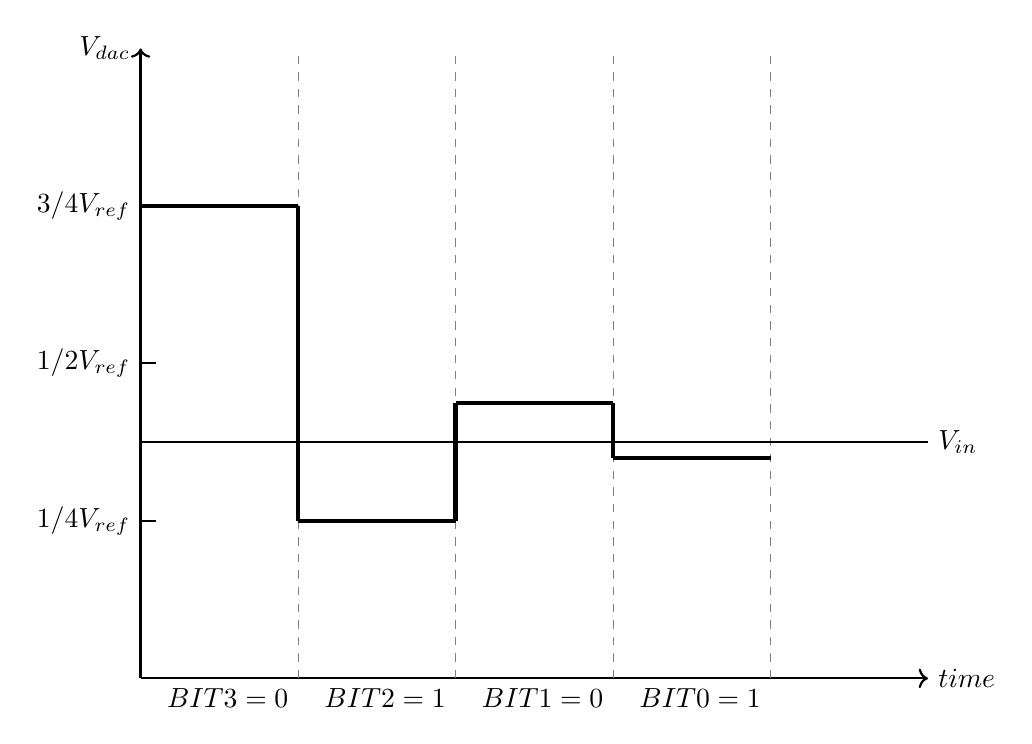
\begin{tikzpicture}
 \draw[thick, ->] (0,0) -- (10,0) node[right]{$time$};
 \draw[thick, ->] (0,0) -- (0,8) node[left]{$V_{dac}$};
 
 \draw[thick] (0,2) node[left]{$1/4 V_{ref}$} -- (0.2,2);
 \draw[thick] (0,4) node[left]{$1/2 V_{ref}$}-- (0.2,4);
 \draw[thick] (0,6) node[left]{$3/4 V_{ref}$}-- (0.2,6);
 
 \draw (2,0) node[anchor= north east] {$BIT3 = 0$};
 \draw (4,0) node[anchor= north east] {$BIT2 = 1$};
 \draw (6,0) node[anchor= north east] {$BIT1 = 0$};
 \draw (8,0) node[anchor= north east] {$BIT0 = 1$};
 \draw [help lines, dashed] (2,0) -- (2,8);
 \draw [help lines, dashed] (4,0) -- (4,8);
 \draw [help lines, dashed] (6,0) -- (6,8);
 \draw [help lines, dashed] (8,0) -- (8,8);
 
 \draw [thick, -] (0,3) -- (10,3)node[right]{$V_{in}$};
 
 \draw [ultra thick, -] (0,6) -- (2,6);
 \draw [ultra thick, -] (2,6) -- (2,2);
 \draw [ultra thick, -] (2,2) -- (4,2);
 \draw [ultra thick, -] (4,2) -- (4,3.5);
 \draw [ultra thick, -] (4,3.5) -- (6,3.5);
 \draw [ultra thick, -] (6,3.5) -- (6,2.8);
 \draw [ultra thick, -] (6,2.8) -- (8,2.8);
 \end{tikzpicture}
 \caption{Example of 4-bit SAR ADC conversion}
 \label{sar:adc}
\end{figure}


\subsubsection{Sample and Hold}
The sample and hold (S/H) is the fist element in the chain. The S/H snatches a value of a analog signal, holds it and digitize it, as shown in Fig. (\ref{sample:hold}). In Fig. (\ref{sample:hold:2})
we can se a simple circuit for a S/H. During \(\phi_{1}\), the switch is on, and the capacitor charges to \(V_{in}\). When the switch closes again $V_{out}$ has the same potential as the capacitor 
at the moment the switch opend \cite{basic-sample-hold}.\\
\\
In the SAR ADC architecture, the function for the sample and hold is to make a stable input calue for the comparator, which compares this input value to the bit sequence, as shown in Fig. (\ref{sar:adc}). 

\begin{figure} 
\centering
 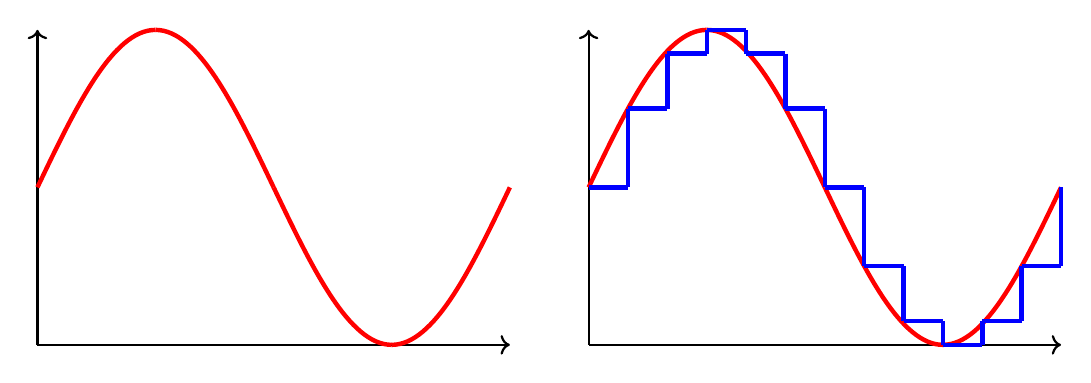
\begin{tikzpicture} 
 %%Denne første modellen er input signalet
    \draw[thick, ->] (0,0)--(6,0);
    \draw[thick, ->] (0,0)--(0,4);
    
    \draw[ultra thick, red] (0,2) sin (1.5,4);
    \draw[ultra thick, red] (1.5,4) cos (3,2);
    \draw[ultra thick, red] (3,2) sin (4.5,0);
    \draw[ultra thick, red] (4.5,0) cos (6,2);
  
  %% Denne andre modellen er samplet signal
    \draw [thick, ->] (7,0)--(13,0);
    \draw [thick, ->] (7,0)--(7,4);
    \draw[ultra thick, red] (7,2) sin (8.5,4);
    \draw[ultra thick, red] (8.5,4) cos (10,2);
    \draw[ultra thick, red] (10,2) sin (11.5,0);
    \draw[ultra thick, red] (11.5,0) cos (13,2);

    \draw[ultra thick, blue] (7,2) -- (7.5,2);
    \draw[ultra thick, blue] (7.5,2) -- (7.5,3);
    \draw[ultra thick, blue] (7.5,3) -- (8,3);
    \draw[ultra thick, blue] (8,3) -- (8,3.7);
    \draw[ultra thick, blue] (8,3.7) -- (8.5,3.7);
    \draw[ultra thick, blue] (8.5,3.7) -- (8.5,4);
    \draw[ultra thick, blue] (8.5,4) -- (9,4);
    \draw[ultra thick, blue] (9,4) -- (9,3.7);
    \draw[ultra thick, blue] (9,3.7) -- (9.5,3.7);
    \draw[ultra thick, blue] (9.5,3.7) -- (9.5,3);
    \draw[ultra thick, blue] (9.5,3) -- (9.5,3);
    \draw[ultra thick, blue] (9.5,3) -- (10,3);
    \draw[ultra thick, blue] (10,3) -- (10,2);
    
    \draw[ultra thick, blue] (10,2) -- (10.5,2);
    \draw[ultra thick, blue] (10.5,2) -- (10.5,1);
    \draw[ultra thick, blue] (10.5,1) -- (11,1);
    \draw[ultra thick, blue] (11,1) -- (11,0.3);
    \draw[ultra thick, blue] (11,0.3) -- (11.5,0.3);
    \draw[ultra thick, blue] (11.5,0.3) -- (11.5,0);
    \draw[ultra thick, blue] (11.5,0) -- (12,0);
    \draw[ultra thick, blue] (12,0) -- (12,0.3);
    \draw[ultra thick, blue] (12,0.3) -- (12.5,0.3);
    \draw[ultra thick, blue] (12.5,0.3) -- (12.5,1);
    \draw[ultra thick, blue] (12.5,1) -- (13,1);
    \draw[ultra thick, blue] (13,1) -- (13,2);
  \end{tikzpicture}
  \caption{Input signal and sampled signal} 
  \label{sample:hold}
\end{figure}

\begin{figure}
\centering
\begin{circuitikz}
\draw (0,0) node[anchor=east]{$v_{in}$}[o-] -- (1,0);
\draw (1,0) to[push button, l=$\phi_{1}$] (3,0);
\draw (3,0) to[C, l=$C$] (3,-2) node[ground] {};
\draw (3,0) -- (5,0)node[anchor=west]{$v_{out}$}[-o];
\end{circuitikz}\caption{Sample and Hold} \label{sample:hold:2}
\end{figure}

\subsubsection{Comparator}
The comparator compares two signals, and outputs either a digital low or high. For a SAR ADC, we compare the sampled reference voltage (\(V_{ref}\)) from the S/H, by the bit sequence from the DAC. 
If the first bit is higher than \(V_{ref}\), the comparator outputs a digital low. Then we know that the sampled value is lower than the value of the first bit. This bit is called the most 
signifiacant bit, shorted as MSB. The calues for the each bit, is discussed in the next subsection.\\
\\
The complexity if the comparator depends on the speed and the accuracy. In some later sections, qe can find the requrements for the circuit and the comparator. Noise in a comparator is a 
concern, and it is therefor important to design the comparator for as low noise as possible. In datacoversion it is often prefered to have a input reffered noise of less than 1 LSB 
(Least Significant Bit). On the other hand, offset is not a concern since it does not affect the overall liniarity \cite{sar-adc-concept}. 

\subsubsection{Digital-to-analog converter}
The digital-to-analog converter (DAC) converts, as the name implies, a digital signal to a analog signal. Depending on the requirements for speed, accuracy, complexity, space and more, it is 
important to find a design that suits the requirements. Table \ref{dac:comparison} shows pros and cons for three different DAC architectures, including R-2R DAC, Resistor string DAC and 
Delta-Sigma DAC \cite{different-dac}. \\
\\
For this project, the R-2R DAC is used. More on why we choosed this architecture is explained in a later chapter. The R-2R is a simple DAC configuration, and consists of only two different 
resistor values hence the name R-2R. Fig. (\ref{r2r:ladder}) shows an example of a 8-bit R-2R ladder, which also is used for this project. The bit sequence into the DAC is controlled by the SAR logic
block, which is briefly discussed in the next subsection. The purpose of the R-2R ladder is to set a specific volage value for each bit. Fist, we test bit 7 (\(b7\)). By using Eq. (\ref{vlsb}), we 
can calculate the output volage of the DAC (\(V_{out}\)) for each bit combination.\\
\\
As an example, we can use \(5V\) as reference volage (\(V_{ref}\)), and set bit 7 to logic high (i.e. 1). All other bits are set to logic low (0). We can now draw an equivalent circuit, 
which is illustrated in Fig. (\ref{example:r2r}). We can se that the output volage is halv the input voltage, i.e 2.5V. 
This bit causes most change to the circutit, and is therefor the MSB. Lets say that the reference voltage from the sample and hold is 1.5V, we notice that the output from the DAC is larger than 1.5V.
This bit is therefor set to low again, and we calculate the output volage for the next bit. It repets these steps intill all the bits are checked. If the output volage is lower than the reference 
volage, the bit is set to logic high, and if the reference volage is higher than the output volage of the DAC, it goes back to logic low.\\
\\
The purpose of the R-2R ladder, is therefor to represent a output value for all bit combinations. In some cases, if the differences between the output volage levels are difficult to separate, 
it is desred to have a operational amplifier with a gain at the output. 

\begin{table}[!ht]
  \centering
 \begin{tabular}{|l|l|l|}
 \hline
			& Pros       			& Cons   			\\ \hline
R-2R DAC 		& - Can achieve high		& - Causing high output 	\\
			& performance INL and DNL	& glitches		   	\\ 
			& - Medium settling time	& - Need HV transistor input	\\
			& capability			&  stage for HV DAC Buffer ->	\\
			& - Low noise R-2R ladder	&  Low BW and setteling		\\
			& - Inherently monotonic	& - Internally, requires high 	\\
			& - Cost Effective		& common mode voltage swing 	\\
			& - Simple to build 		& output amp		 	\\ \hline
Resistor		& - No need for trimming	& - Requires 2\^N -1 matching 	\\
String DAC		& - Good DNL performance	& resistors			\\
			& - Low Glitch Energy		& - Resolution is limited	\\ 
			& 				& - Size can grow with 		\\
			&				& resolution requirement	\\
			& 				& - High resolution is achieved \\
			&				& by pipeline-like		\\
			& 				& architectures which 		\\
			&				& compromises monotonocity	\\ \hline
Delta-Sigma		& - High resolution		& - Settling time \(\sim\) 2ms	\\
DAC			& - Low Power			& - Long Latency		\\
			& - Voltage output		& -  Not optimized for DC	\\
			& - Good Linearity		&				\\
			& - Low Cost			&				\\
			& - In Audio: moving noise	&				\\
			& out of audible range		&				\\ \hline
 \end{tabular}
 \caption{Comparation of different ADCs}
 \label{dac:comparison}
 \end{table}
 
 \begin{figure}
  \centering
  \ctikzset{bipoles/length = 1cm}
  \begin{circuitikz}[scale = 0.5]
   \draw (0,0) -- (1,0);
   \draw (0,0) -- (0,-1) to[R, l={$2R$}] (0,-3) node[ground]{};
   \draw (0,0) -- (0,1) to[R, l={$2R$}] (0,3) -- (0,4)[-o,]node[above]{$b0$};
   \draw (1,0) to[R, l={$R$}] (3,0) -- (4,0);
   \draw (3.5,0) -- (3.5,1) to[R, l={$2R$}] (3.5,3) -- (3.5,4)[-o]node[above]{$b1$};
   \draw (4,0) to[R, l={$R$}] (6,0) -- (7,0);
   \draw (6.5,0) -- (6.5,1) to[R, l={$2R$}] (6.5,3) -- (6.5,4)[-o]node[above]{$b2$};
   \draw (7,0) to[R, l={$R$}] (9,0) -- (10,0);
   \draw (9.5,0) -- (9.5,1) to[R, l={$2R$}] (9.5,3) -- (9.5,4)[-o]node[above]{$b3$};
   \draw (10,0) to[R, l={$R$}] (12,0) -- (13,0);
   \draw (12.5,0) -- (12.5,1) to[R, l={$2R$}] (12.5,3) -- (12.5,4)[-o]node[above]{$b4$};
   \draw (13,0) to[R, l={$R$}] (15,0) -- (16,0);
   \draw (15.5,0) -- (15.5,1) to[R, l={$2R$}] (15.5,3) -- (15.5,4)[-o]node[above]{$b5$};
   \draw (16,0) to[R, l={$R$}] (18,0) -- (19,0);
   \draw (18.5,0) -- (18.5,1) to[R, l={$2R$}] (18.5,3) -- (18.5,4)[-o]node[above]{$b6$};
   \draw (19,0) to[R, l={$R$}] (21,0);
   \draw (21.5,0) -- (21.5,1) to[R, l={$2R$}] (21.5,3) -- (21.5,4)[-o]node[above]{$b7$};
   \draw (21,0) -- (23,0)[-o] node[right]{$V_{out}$};
  \end{circuitikz}
  \caption{Example of 8-bit R-2R ladder}
  \label{r2r:ladder}
 \end{figure}
 
\begin{equation}\label{vlsb}
 V_{LSB} = V_{ref} \cdot \frac{1}{2^{N}}
\end{equation}

\begin{equation}
 V_{Max} = V_{ref} \cdot \frac{2^{N}-1}{2^{N}}
\end{equation}

\begin{equation}
 BinVal = \sum_{i=0}^{N-1} 2^{i} \cdot b_{i}
\end{equation}

\begin{equation}
 V_{out} = V_{LSB} \cdot BinVal
\end{equation}

\begin{figure}
\centering
 \begin{circuitikz}
 \draw (0,0)[o-]  node[left]{$V_{ref}$} -- (1,0);
 \draw (1,0)to[R, l=$2R$] (3,0) -- (5,0)[-o] node[right]{$V_{out}$};
 \draw (3.5,0) -- (3.5,-1) to[R, l={$2R$}] (3.5,-3) node[ground]{};
 \end{circuitikz}
 \caption{R-2R equivalent circuit is \(b7\) is set}
 \label{example:r2r}
\end{figure}

\subsubsection{Logic}
The SAR logic block, is the ``brain'' of the circuit. The scope of the project is not to design this block, and is therefor not discussed in detail here. The block contains three inputs and 
two outputs, where one of the outputs is a bit sequence of total 8-bits. The block with its I/Os are shown in Fig. (\ref{sar:logic}). Each I/O is briefly discussed under, and Fig. (\ref{timing_sar})
shows a typical timing diagram for the SAR logic block.
\begin{figure}[!ht]
 \centering
 \begin{tikzpicture}
  \draw [thick] (0,0) rectangle (4,4);
  \draw[thick] (-2,1)[o-] node[left]{$keep$} -- (0,1);
  \draw (-2,2)[o-]node[left]{$SoC$} -- (0,2);
  \draw (-2,3)[o-]node[left]{$clk$} -- (0,3);
  \draw (4,1) -- (6,1)[-o]node[right]{$done$};
  \draw (4,3) -- (6,3)[-o]node[right]{$b<7:0>$};
 \end{tikzpicture}
 \caption{SAR logic block}
 \label{sar:logic}
\end{figure}
\begin{figure}[!ht]
 \centering
 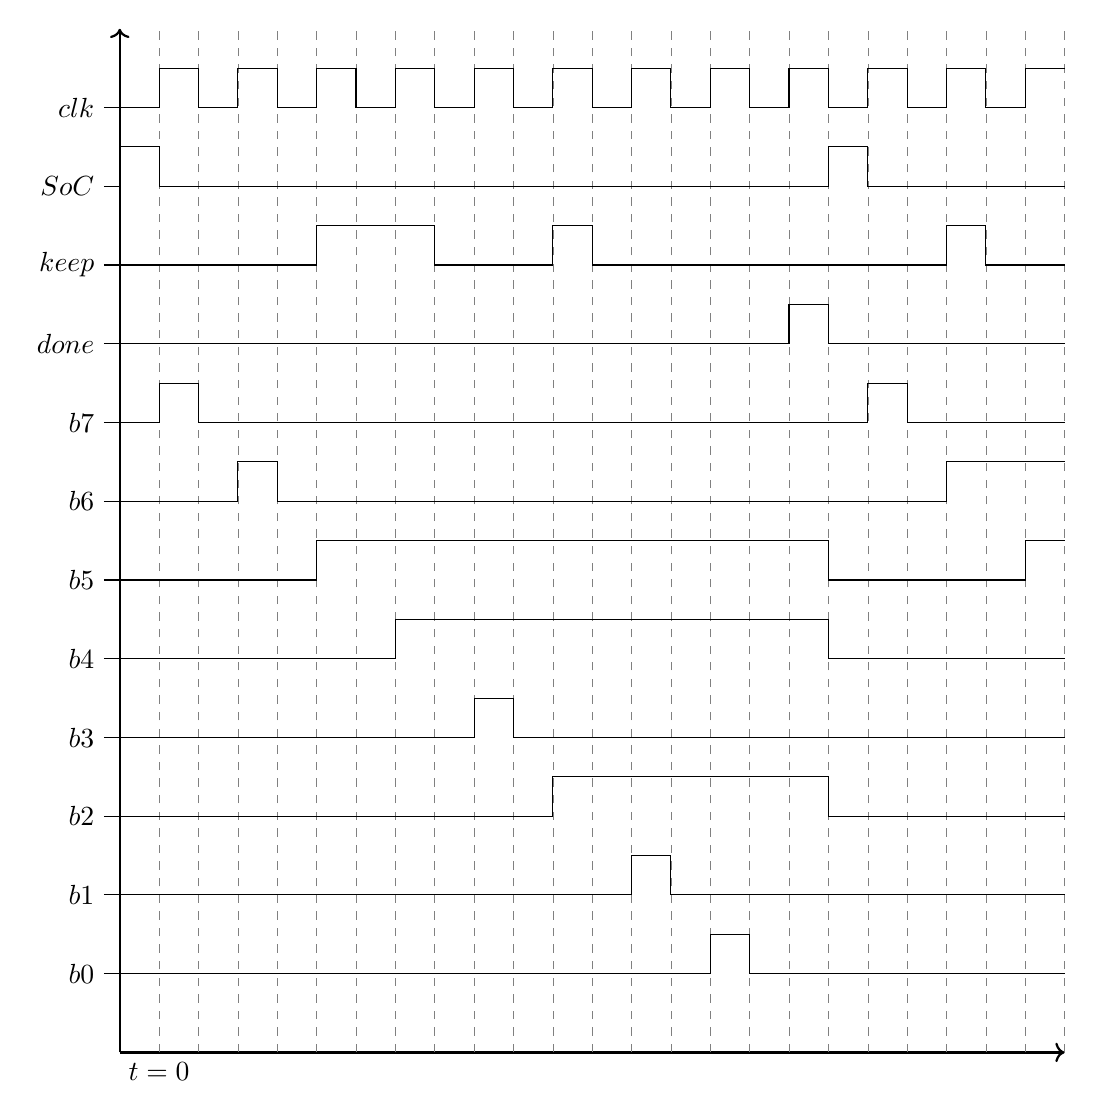
\begin{tikzpicture}
  \draw[thick, ->](0,0) -- (12,0);
  \draw[thick, ->](0,0) -- (0,13);
  
  \draw (0.5,0) node[anchor= north] {$t=0$};
  
  \draw [help lines, dashed] (0.5,0) -- (0.5,13);
  \draw [help lines, dashed] (1,0) -- (1,13);
  \draw [help lines, dashed] (1.5,0) -- (1.5,13);
  \draw [help lines, dashed] (2,0) -- (2,13);
  \draw [help lines, dashed] (2.5,0) -- (2.5,13);
  \draw [help lines, dashed] (3,0) -- (3,13);
  \draw [help lines, dashed] (3.5,0) -- (3.5,13);
  \draw [help lines, dashed] (4,0) -- (4,13);
  \draw [help lines, dashed] (4.5,0) -- (4.5,13);
  \draw [help lines, dashed] (5,0) -- (5,13);
  \draw [help lines, dashed] (5.5,0) -- (5.5,13);
  \draw [help lines, dashed] (6,0) -- (6,13);
  \draw [help lines, dashed] (6.5,0) -- (6.5,13);
  \draw [help lines, dashed] (7,0) -- (7,13);
  \draw [help lines, dashed] (7.5,0) -- (7.5,13);
  \draw [help lines, dashed] (8,0) -- (8,13);
  \draw [help lines, dashed] (8.5,0) -- (8.5,13);
  \draw [help lines, dashed] (9,0) -- (9,13);
  \draw [help lines, dashed] (9.5,0) -- (9.5,13);
  \draw [help lines, dashed] (10,0) -- (10,13);
  \draw [help lines, dashed] (10.5,0) -- (10.5,13);
  \draw [help lines, dashed] (11,0) -- (11,13);
  \draw [help lines, dashed] (11.5,0) -- (11.5,13);
  \draw [help lines, dashed] (12,0) -- (12,13);
  
  \draw(-0.2,1) node[left]{$b0$} -- (0,1);
  \draw(-0.2,2) node[left]{$b1$} -- (0,2);
  \draw(-0.2,3) node[left]{$b2$} -- (0,3);
  \draw(-0.2,4) node[left]{$b3$} -- (0,4);
  \draw(-0.2,5) node[left]{$b4$} -- (0,5);
  \draw(-0.2,6) node[left]{$b5$} -- (0,6);
  \draw(-0.2,7) node[left]{$b6$} -- (0,7);
  \draw(-0.2,8) node[left]{$b7$} -- (0,8);
  \draw(-0.2,9) node[left]{$done$} -- (0,9);
  \draw(-0.2,10) node[left]{$keep$} -- (0,10);
  \draw(-0.2,11) node[left]{$SoC$} -- (0,11);
  \draw(-0.2,12) node[left]{$clk$} -- (0,12);
  
  \draw(0,12)--(0.5,12)--(0.5,12.5)--(1,12.5)--(1,12)--(1.5,12)--(1.5,12.5)--(2,12.5)--(2,12)--(2.5,12)--(2.5,12.5)--(3,12.5)--(3,12)--(3.5,12)--(3.5,12.5)--(4,12.5)--
  (4,12)--(4.5,12)--(4.5,12.5)--(5,12.5)--(5,12)--(5.5,12)--(5.5,12.5)--(6,12.5)--(6,12)--(6.5,12)--(6.5,12.5)--(7,12.5)--(7,12)--(7.5,12)--(7.5,12.5)--(8,12.5)--(8,12)--(8.5,12)--
  (8.5,12.5)--(9,12.5)--(9,12)--(9.5,12)--(9.5,12.5)--(10,12.5)--(10,12)--(10.5,12)--(10.5,12.5)--(11,12.5)--(11,12)--(11.5,12)--(11.5,12.5)--(12,12.5);
  \draw(0,11.5)--(0.5,11.5)--(0.5,11)--(9,11)--(9,11.5)--(9.5,11.5)--(9.5,11)--(10,11)--(12,11);
  \draw(0,10)--(2.5,10)--(2.5,10.5)--(4,10.5)--(4,10)--(5.5,10)--(5.5,10.5)--(6,10.5)--(6,10)--(10.5,10)--(10.5,10.5)--(11,10.5)--(11,10)--(12,10);
  \draw(0,9)--(8.5,9)--(8.5,9.5)--(9,9.5)--(9,9)--(12,9);
  \draw(0,8)--(0.5,8)--(0.5,8.5)--(1,8.5)--(1,8)--(9.5,8)--(9.5,8.5)--(10,8.5)--(10,8)--(12,8);
  \draw(0,7)--(1.5,7)--(1.5,7.5)--(2,7.5)--(2,7)--(10.5,7)--(10.5,7.5)--(11,7.5)--(12,7.5);
  \draw(0,6)--(2.5,6)--(2.5,6.5)--(9,6.5)--(9,6)--(11.5,6)--(11.5,6.5)--(11.5,6.5)--(12,6.5);
  \draw(0,5)--(3.5,5)--(3.5,5.5)--(9,5.5)--(9,5)--(12,5);
  \draw(0,4)--(4.5,4)--(4.5,4.5)--(5,4.5)--(5,4)--(12,4);
  \draw(0,3)--(5.5,3)--(5.5,3.5)--(9,3.5)--(9,3)--(12,3);
  \draw(0,2)--(6.5,2)--(6.5,2.5)--(7,2.5)--(7,2)--(12,2);
  \draw(0,1)--(7.5,1)--(7.5,1.5)--(8,1.5)--(8,1)--(12,1);
 \end{tikzpicture}
 \caption{Typical timing diagram for the SAR logic block}
 \label{timing_sar}
\end{figure}
\newline
\textbf{Signal clk:}\\
The clock signal (\(clk\)) is a contiues signal that cycles at a duty cycle of 50\% This signal is controlled by the microcontroller.\\
\\
\textbf{Signal SoC:}\\
Start of conversion (\(SoC\)) is the first signal that happens. This is the trigger signal that starts the bit counting, and happens when the \(SoC\) goes logic low. It stays low during the 
whole couning period. When the last bit is pulsed, it waits for a interrupt from the end of conversion (EoC), which is named \(done\) in this block. After \(done\) is pulsed, \(SoC\) goes
high for one period, and then it starts again.\\
\\
\textbf{Signal done:}\\
As mentrioned above, the \(done\) signal happens when all the bits has cycled once. The \(done\) signal indicates that the round is finnished, and the \(SoC\) can go high, and start a new turn.\\
\\
\textbf{Signal b<7:0>:}\\
For this system, there are total 8-bits. All of these bits happens at different time, starting at the MSB and ending at the LSB. For more detailed information about how these bits operate, see
the section for the DAC.\\
\\
\textbf{Signal keep:}\\
The \(keep\) signal is the input to the SAR logic block from the comparator. If the DAC output is higher than the reference voltage from the S/H, the comparator outputs a logic low, indicating
that the represented bit not will be kept. If the comparator outputs a logic high, the DAC output is lower than the reference voltage, and the bis is kept. More detaild information on how this works, 
can be found in the subsention for the comparator.  



\subsection{Requirements}
In todays technologies, it is important to consume as low power as possible, and be as fast as possible. Due to this, we are going to design a SAR ADC which are capable 
of running with a powersupply of 1.2 V and have sampling frequency of 1 MHz. The overall requirements are listed bellow.\\
\textbf{SAR ADC}
\begin{itemize}
 \item Input sampling rate: 1 M samples/s
 \item Output resolution: 8 bits
 \item Supply voltage: \(V_{DD} = 1.2 V\), and \(V_{SS} = 0 V\)
 \item No missing codes
 \item Monotonic
\end{itemize}
\textbf{DAC}
\begin{itemize}
 \item Sampling rate: 8 M samples/s
 \item Resolution: 8 bits
 \item Supply voltage: \(V_{DD} = 1.2 V\), and \(V_{SS} = 0 V\)
 \item DNL < \(\pm\) 0.5 LSB
 \item INL < \(\pm\) 0.5 LSB
 \item \(V_{OUT(P\_P)} \geq 0.6 V\)
 \item \(C_{load} = 50 fF\)
\end{itemize}
\textbf{Comparator}
\begin{itemize}
 \item Delay \(\leq\) 0.5 clock cycle
 \item Supply Voltage: \(V_{DD} = 1.2V\) and \(V_{SS} = 0V\) 
 \item Offset < 0.5 LSB
 \item Gain > \(V_{DD}/V_{ref}/2^{n}\)
 \item \(C_{load} = 50 fF\)
\end{itemize}

\section{Planning the project} 
Before stating the work on the shematics, we searched for litterature in textbooks and on the internet. There was also a mandatory handin for a prestudy for comparing different ADC types. This 
comparison is losted in Table (\ref{comp:adc}) \cite{forstudie}. There has also been carried out a status report during the prosject. The total circuit was discussed at this stage of the prosject.
After this report, there has beed done a lot of changes to the circuit. These changes are discussed in detail in the nest section. 

\begin{table}[!ht]
 \centering
 \begin{tabular}{|l|l|l|l|l|}
  \hline
                   & SAR        & Flash   & Sigma-Delta  & Integrating          \\ \hline
  Conversion speed & Low-medium & Fast    & Low          & Depending on 	\\
		   &	        &	  &		 & reolution and 	\\
		   &		&	  &		 & clock 		\\ \hline
  Sampling rate    & Nyquist    & Nyquist & Oversampling & Nyquist              \\ \hline
  Area             & Low        & High    & Medium       &                      \\ \hline
 \end{tabular}
 \caption{Comparation of different ADCs}
 \label{comp:adc}
\end{table}

\newpage
\section{Results} 
In order to get a god overview of the different parts of the total system, each block in the system is separated into sections. As a summary all the blocks are duscussed together as a final, and 
total system. To be sure that every part works as i should, we made own working directoris for each part. The naming for the blocks were kept consequently, so that there would not create any problem. 
To get a better overview for the reader, we have listed the hierarchy bellow. Note that some of the blocks has a number at the end of the name. This indicates the verson. 
\begin{itemize}
 \item SIM\_SAR\_system\_3
 \begin{itemize}
  \item SAR\_system\_3
 \end{itemize}
 \item SIM\_sample\_hold\_3
 \begin{itemize}
  \item sample\_hold\_3
 \end{itemize}
 \item SIM\_comparator\_rail2rail\_external\_current
 \begin{itemize}
  \item comparator\_rail2rail\_external\_current
 \end{itemize}
 \item SIM\_dac\_real\_res
  \begin{itemize}
  \item dac\_real\_res
 \end{itemize}
 \item SIM\_SAR\_logic
  \begin{itemize}
  \item SAR\_logic
 \end{itemize}
 \item SIM\_SR\_latch
  \begin{itemize}
  \item SR\_latch
 \end{itemize}
 \item SIM\_output\_buffers
  \begin{itemize}
  \item output\_buffers
 \end{itemize}
\end{itemize}
In addtion, there are also one more block, that was created when we simulated the layout. Since the SAR logic block is not supporting layout, we had to take this block out of the whole system, 
and simulate it separately. These files are called:
\begin{itemize}
 \item SIM\_SAR\_system\_3\_u\_sar\_logic
 \begin{itemize}
  \item SAR\_system\_3\_u\_sar\_logic
 \end{itemize}
\end{itemize}
The \textit{Results} section is divided into subsections, where each subsection repressent each block in the system. Each sub section contains a simulation part and a component part. 
The component part is the actual schematic for the block. The subsentions is ranged in the same order as in the introduction. In the end, the addtional blocks, such as \textit{SR latch}, and 
\textit{output buffers} are discussed. For the thery of each block, we refers to Section 1, Introduction. 

%%%%%%%%%%%%%%%%%%%%%%%%%%%%%%%%%%%%%%%%%%%%%%%%%%%%%%%%%%%%%%%%%%%%%%%%%%%%%%%
%% Sample and hold
%%%%%%%%%%%%%%%%%%%%%%%%%%%%%%%%%%%%%%%%%%%%%%%%%%%%%%%%%%%%%%%%%%%%%%%%%%%%%%%
\subsection{Sample and hold}
In our design we have a sample and hold circuit that tracks the input signal. When the circuit should perform a conversion the signal is held constant.
\subsubsection{Implementation}
Our first implementation was a simple nmos transistor as the switch. In this case we was not able to get a clean signal when the signal was grater than VDD/2. 
Simulations showed that the signal started to be distorted already at 700mV (about 58\% of VDD).

Since we have aimed at full range performance of our circuit we needed a better switch and changed the switch implementation into a transmission gate. 

We also included a operational amplifier in our design but realized that our comparator had so high input impedance that this was not needed. The input capacitance of the 
comparator is sufficiently small so the stored charge in the capacitor (and hence the voltage over the capacitor) is not very distorted during comparison.


The functional implementation is illustrated in figure (\ref{sample:hold:design}) and the actual implementation is in the appendix. 
The function of the input \(\phi\) is listed in table \ref{table:sample_and_hold:function}.


%---------------------------- SH Circuit -------------------------------
\begin{figure}[!ht]
\centering
 \begin{circuitikz} \draw 
  (0,0)node[anchor=east]{$v_{in}$} to[short, o-] (2,0)
  (1.5,2) node[not port](not1){}
  (0,2)node[anchor=east]{$\phi$} to[short, o-](1,2) -- (not1.in)
  
  (2,0) to[Tnmos, n=n1] (4,0)
  (not1.out) -| (n1.G)
  (2,0) to[Tpmos, n=p1, mirror](4,0) -- (5,0)
  (not1.in) |- (p1.G)
  
  (5,0) to[C, l=$C$] (5,-2) node[ground] {}
  (5,0) -- (7,0)node[anchor=west]{$v_{out}$}[-o]
 ;\end{circuitikz}
\caption{Sample and Hold design} 
\label{sample:hold:design}
\end{figure}

%---------------------------- SH functional table --------------------------
\begin{table}[]
\centering
\begin{tabular}{|l|l|}
\hline
\(\phi\) & Function \\ \hline
0   & Track    \\ \hline
1   & Hold     \\ \hline
\end{tabular}
\caption{Sample and Hold function selection}
\label{table:sample_and_hold:function}
\end{table}
\subsubsection{Simulation}



%%%%%%%%%%%%%%%%%%%%%%%%%%%%%%%%%%%%%%%%%%%%%%%%%%%%%%%%%%%%%%%%%%%%%%%%%%%%%%%
%% Comparator
%%%%%%%%%%%%%%%%%%%%%%%%%%%%%%%%%%%%%%%%%%%%%%%%%%%%%%%%%%%%%%%%%%%%%%%%%%%%%%%
\subsection{Comparator}
\subsubsection{SIM\_comparator\_rail2rail\_external\_current}
\subsubsection{comparator\_rail2rail\_external\_current}

\begin{figure}[!ht]
\centering
\ctikzset{bipoles/length = 0.8cm}
 \begin{circuitikz}
  \draw[yscale=0.8, xscale=0.6]
  (3,5) -- (0,5) to[Tpmos, n=p1](0,3) to[R] (0,0) to[Tnmos, n=n1] (0,-1.5) node [ground]{}
  (3,5) to[Tpmos, n=p2, mirror] (3,3) (p2.G) -- (p1.G)node[circ]{} |- (p1.S)node[circ]{}
  
  (3,5) -- (6,5) to[Tpmos, n=p3, mirror](6,3) -- (6,2.5) (p3.G) |- ($(p3.S)-(0,0.5)$)node[circ]{}
  (6,5) -- (8,5) to[Tpmos, n=p4, mirror] (8,3)  ($(p3.S)-(0,0.5)$) -| (p4.G)
  (8,5) -- (9,5) to[Tpmos, n=p5] (9,3) (p4.S)node[circ]{} -- ($(p5.G)-(1.63,1.46)$)node[circ]{} ($(p4.G)-(-1.63,1.46)$)node[circ]{} -- (p5.S)node[circ]{}
  (9,5) -- (11,5) to[Tpmos, n=p6] (11,3) -- (11,2.5) (p5.G) |- ($(p6.S)-(0,0.5)$) (p6.G) |- ($(p6.S)-(0,0.5)$)node[circ]{}
  
  (4.37,2) to[Tnmos, n=n2, mirror] (4.37,0.5) (n2.S) -- ($(p3.G)-(0,1.46)$)node[circ]{} (n2.G)to[short, -o]($(n2.G)-(0.8,0)$)node[anchor=east]{In}
  (12.63,2) to[Tnmos, n=n7](12.63,0.5) (n7.S) -- ($(p6.G)-(0,1.46)$)node[circ]{} (n7.D) -- (n2.D) (n7.G)to[short, -o]($(n7.G)+(1,0)$)node[anchor=west]{Ref}
  
  (4.37,-3) to[Tpmos, n=p7, mirror] (4.37,-4.5) (n2.G) -- (p7.G)
  (12.63,-3) to[Tpmos, n=p8](12.63,-4.5) (p8.G) -- (n7.G) (p7.D) -- (p8.D) 
  
  (8.5,0) to[Tnmos, n=n4, mirror](8.5,-1.5)node[ground]{} (n1.G) -- (n4.G) (n4.S) -- ($(n2.D)+(4.13,0)$)node[circ]{} 
  
  (4.37,-5) to[Tnmos, n=n5](4.37,-6.5) node[ground]{} (p7.S) -- (n5.S) (n5.G)node[circ]{} |- (n5.S)node[circ]{}
  (7.37,-5) to[Tnmos, n=n6, mirror](7.37,-6.5) node[ground]{} (n5.G) -- (n6.G) (n6.S) -- (7.37,1)node[circ]{} -- ($(p5.G)-(1.63,1.46)$) -- ($(p5.G)-(0,1.46)$) 
  (9.63,-5) to[Tnmos, n=n8](9.63,-6.5) node[ground]{} (n8.S) -- (9.63, 1)node[circ]{} -- ($(p4.G)-(-1.63,1.46)$) -- ($(p4.G)-(0,1.46)$)
  (12.63,-5) to[Tnmos, n=n9, mirror](12.63,-6.5) node[ground]{} (n8.G) -- (n9.G) (n9.G)node[circ]{} |- (n9.S)node[circ]{} (n9.S) -- (p8.S)
  (p2.S) |- ($(p8.D)+(-4,0.5)$) -- ($(p8.D)-(4,0)$)node[circ]{} 
  
  (11,5) -| (17,4) to[Tpmos, n=p9, mirror](17,2) (p9.G) -- ($(p6.G)-(0,1)$)node[circ]{}
  (17,0) to[Tnmos, n=n10, mirror](17,-2)node[ground]{} (n10.S) -- (p9.S) (n10.G) |- (n4.G)
  (17,5) -| (20,3) to[Tpmos, n=p10, mirror](20,1) (p10.S) to[short, -o]($(p10.S)+(1,0)$)node[anchor=west]{OUT} 
  (20,1) to[Tnmos, n=n11, mirror](20,-1)node[ground]{} (p10.G) -- (n11.G) ($(n11.G)+(0,1)$)node[circ]{} -- ($(n10.S)+(0,1.04)$)node[circ]{}
  
  (20,5) to[short, -o] (21,5)node[anchor=west]{$V_{DD}$}
 ;\end{circuitikz}
 \caption{Comparator design}
 \label{comp:design}
\end{figure}


\subsection{Digital-to-analog converter}
\subsubsection{Implementation}
The implementation for the DAC is shown in Fig. (\ref{r2r:ladder:real}). After a long study on different types of DAC, we decided to use a R-2R implementation. This decision was mainly due to 
complexity. A resistor string implementation has been considered, but this implementation is so complex for a 8-bit DAC. The resistor string needs a lot of digital logic circuit, but the main 
reason is the large amount of resistors needed. For a 8-bit system, it is required to have \(2^N\) resistor \cite{carusone}. This means that there would be 256 resistors. Due to this large amount of resistor, 
this circuit has not been simulated and tested. An other DAC architecture that has been considered, is a Charge-Redistribution Switched-Capacitor converter. The advantage for using this circuit 
is the elimination of all the resistors. In stead, this implementation uses capacitors, which is much smaller in size when talking about layout. An other advantage is low power consumption if the
circuit is modeled properly. The Charge-Redistribution Switched-Capacitor converter has been tested and simulated. We founded this circuit difficult to model properly, and we experienced 
timing issues and some problems modeling the logic. We used a lot of time modeling this circuit without any succeed.\\
%%---------------DAC
 \begin{figure}[!ht]
   \centering
   \ctikzset{bipoles/length = 1cm}
   \begin{circuitikz}[scale = 0.5]\draw
    (0,5) node[not port, rotate=270](not2){}
    (3.5,5) node[not port, rotate=270](not3){}
    (6.5,5) node[not port, rotate=270](not4){}
    (9.5,5) node[not port, rotate=270](not5){}
    (12.5,5) node[not port, rotate=270](not6){}
    (15.5,5) node[not port, rotate=270](not7){}
    (18.5,5) node[not port, rotate=270](not8){}
    (21.5,5) node[not port, rotate=270](not9){}
    (0,8) node[not port, rotate=270](not10){}
    (3.5,8) node[not port, rotate=270](not11){}
    (6.5,8) node[not port, rotate=270](not12){}
    (9.5,8) node[not port, rotate=270](not13){}
    (12.5,8) node[not port, rotate=270](not14){}
    (15.5,8) node[not port, rotate=270](not15){}
    (18.5,8) node[not port, rotate=270](not16){}
    (21.5,8) node[not port, rotate=270](not17){}
    (0,0) -- (1,0)
    (0,0) -- (0,-1) to[R, l={$2R$}] (0,-3) node[ground]{}
    (0,0) -- (0,1) to[R, l={$2R$}] (0,3) -- (not2.out) (not2.in) --(not10.out) (not10.in) to[short, -o](0,10)node[above]{$b0$}
    (1,0) to[R, l={$R$}] (3,0) -- (4,0)
    (3.5,0) -- (3.5,1) to[R, l={$2R$}] (3.5,3) -- (not3.out) (not3.in) --(not11.out) (not11.in) to[short, -o](3.5,10)node[above]{$b1$}
    (4,0) to[R, l={$R$}] (6,0) -- (7,0)
    (6.5,0) -- (6.5,1) to[R, l={$2R$}] (6.5,3) -- (not4.out) (not4.in) --(not12.out) (not12.in) to[short, -o](6.5,10)node[above]{$b2$}
    (7,0) to[R, l={$R$}] (9,0) -- (10,0)
    (9.5,0) -- (9.5,1) to[R, l={$2R$}] (9.5,3) -- (not5.out) (not5.in) --(not13.out) (not13.in) to[short, -o](9.5,10)node[above]{$b3$}
    (10,0) to[R, l={$R$}] (12,0) -- (13,0)
    (12.5,0) -- (12.5,1) to[R, l={$2R$}] (12.5,3) -- (not6.out) (not6.in) --(not14.out) (not14.in) to[short, -o](12.5,10)node[above]{$b4$}
    (13,0) to[R, l={$R$}] (15,0) -- (16,0)
    (15.5,0) -- (15.5,1) to[R, l={$2R$}] (15.5,3) -- (not7.out) (not7.in) --(not15.out) (not15.in) to[short, -o](15.5,10)node[above]{$b5$}
    (16,0) to[R, l={$R$}] (18,0) -- (19,0)
    (18.5,0) -- (18.5,1) to[R, l={$2R$}] (18.5,3) -- (not8.out) (not8.in) --(not16.out) (not16.in) to[short, -o](18.5,10)node[above]{$b6$}
    (19,0) to[R, l={$R$}] (21,0)
    (21.5,0) -- (21.5,1) to[R, l={$2R$}] (21.5,3) -- (not9.out) (not9.in) --(not17.out) (not17.in) to[short, -o](21.5,10)node[above]{$b7$}
    (21,0) to[short, -o] (23,0)node[right]{$V_{out}$}
  ; \end{circuitikz}
   \caption{Implemented 8-bit R-2R ladder}
   \label{fig:r2r:ladder:real}
  \end{figure}
%%--------------------
\newline
In the ending, we ended up with the R-2R ladder. Many examples of this circuit is modeled with a operational amplifier. This is because the R-2R requires a high impedance at the output in order to
work properly. This is not a problem in out design, because the comparator has a very high impedance, meaning that it would be a waste of space and time modeling a extra operational amplifier at
the output. In Fig. (\ref{r2r:ladder:real}), there are implemented two inverters at the input for every bit. This is because we experienced that the SAR logick block did not output logic high at
1.2V, but 1V instead. It is important for the systems accuracy to have full swing at the DAC output. Therefor, we implemented two inverters at the input, the second for not inverting the signal. 
The size of the resistors is set to be 380k\(\ohm\) and 760k\(\ohm\). More on why these sizes are used, is discussed in the simulation section. 

\subsubsection{Simulation}
\begin{figure}
 \centering
 \begin{circuitikz}
  
 \end{circuitikz}

\end{figure}

 
\subsection{SAR logic}
\subsubsection{SIM\_SAR\_logic}
\subsubsection{SAR\_logic}

\subsection{SR latch}
\subsubsection{SIM\_SR\_latch}
\subsubsection{SR\_latch}

%%------ SR LATCH
\begin{figure}
\centering
 \begin{circuitikz}[yscale=1, xscale=1]\draw
  
  
  (2,3) node[nor port](nor1){}
  (nor1.in 1)--($(nor1.in 1)-(1,0)$)node[anchor=east]{\(R\)}
  
  (2,0) node[nor port](nor2){}
  (nor2.in 2)--($(nor2.in 2)-(1,0)$)node[anchor=east]{\(S\)}
  
  (nor1.out) -- ($(nor1.out)+(1,0)$) -- ($(nor2.in 1)+(0,0.6)$) -| (nor2.in 1) (nor1.out)to[short, -o](4,3) node[anchor=west]{\(Q\)}
  (nor2.out) -- ($(nor2.out)+(1,0)$) -- ($(nor1.in 2)-(0,0.6)$) -| (nor1.in 2) (nor2.out)to[short, -o](4,0) node[anchor=west]{\(\bar Q\)}
 ;\end{circuitikz}
 \caption{SR latch}
 \label{sr:latch}
\end{figure}
%%------------

\begin{table}[]
\centering

\begin{tabular}{|l|l|l|l|}
\hline 
			 &			    &			       &			   \\ 	
\(S\)			 & \(R\)		    & \(Q\)		       & \(\bar Q\)		   \\ \hline
0                        & 0                        & NC            	       & NC             	   \\ \hline
0                        & 1                        & 0                        & 1                         \\ \hline
1                        & 0                        & 1                        & 0                         \\ \hline
1                        & 1                        & 0                        & 1                         \\ \hline
\end{tabular}
\caption{My caption}
\label{my-label}
\end{table}

\subsection{Output buffers}
\subsubsection{SIM\_output\_buffers}
\subsubsection{output\_buffers}

\subsection{SAR system}
\subsubsection{SIM\_SAR\_system\_3}
\subsubsection{SAR\_system\_3}


\section{Discussion and conclusion}
\section{Discussion}
\subsection{Proposal of improvement}
\section{Conclusion}

\section{Punkter som kanskje skal med}
Critical parts in SAR ADCs 

\begin{itemize}
 \item Comparator
 \item DAC
\end{itemize}

SAR ADCs limitations:

\begin{itemize}
 \item The settling time is the DAC, whick must settle within the resolution of the overall converterm for example, 1/2 LSB (Least significant bit)
 \item The comparator, which must resolve small differences in $V_{in}$ and $V_{DAC}$ within the specified time
 \item The logic overhead

 \end{itemize}
Comparator:

\begin{itemize}
 \item The comparator does not effect the overall linearity 
\end{itemize}


\begin{appendices}
\chapter{Software and instrument overview}
\end{appendices}

\printbibliography{}

\end{document}

% TABELL FOR SAMMENLIGNING AV FORSKJELLIGE ADC




% --------------------------------------------------------------------
% Fotnote eksempel
% Hei \footnote{\url{http://www.google.fi/}}
% --------------------------------------------------------------------
% Figur eksempel
% \begin{figure}[!ht]
%   \centering
%     \includegraphics[width=0.5\textwidth]{filplassering}
%     \caption{Bildetekst}
%     \label{fig:}
% \end{figure}
% ---------------------------------------------------------------------
% For en mer bestemt plassering:
% 
% \begin{wrapfigure}{r}{0.5\textwidth}
%   \begin{center}
%     \includegraphics[width=0.48\textwidth]{filplassering}
%   \end{center}
%   \caption{Bildetekst}
%   \label{fig:}
% \end{wrapfigure}
% 
% Plasseringer for bilde:
% r 	R 	right side of the text
% l 	L 	left side of the text
% i 	I 	inside edge–near the binding (in a twoside document)
% o 	O 	outside edge–far from the binding
% ----------------------------------------------------------------------
% For å innkludere skjematiske tegninger:
%
%\begin{circuitikz}[scale=1.25]

% \draw (-1,0) node[anchor=east] {} to [short, *-*] (1,0);
% \draw (-1,2) node[anchor=east] {} to [inductor, *-*,  l=$\Delta x L$] (1,2);
% \draw (-1,0) to [open, l=$\cdots$] (-1,2);    
% \draw (3, 0) to (1, 0) to [capacitor, l=$\Delta x C$, *-*] (1, 2) to [inductor, *-*, l=$\Delta x L$] (3, 2);
% \draw (5, 0) to (3, 0) to [capacitor, l=$\Delta x C$, *-*] (3, 2) to [inductor, *-*, l=$\Delta x L$] (5, 2);
% \draw (7, 0) to (5, 0) to [capacitor, l=$\Delta x C$, *-*] (5, 2) to [inductor, *-*, l=$\Delta x L$] (7, 2);
% \draw (9, 0) to (7, 0) to [capacitor, l=$\Delta x C$, *-*] (7, 2) to [inductor, *-*, l=$\Delta x L$] (9, 2);
% \draw (9,0) node[anchor=east] {} to [short, *-*] (9,0);
% \draw (10,0) to [open, l=$\cdots$] (10,2);

% \end{circuitikz}
% ----------------------------------------------------------------------
% Paranteser
% 
% \big( \Big( \bigg( \Bigg( 	
% \big] \Big] \bigg] \Bigg] 	
% \big\{ \Big\{ \bigg\{ \Bigg\{ 	
% \big \langle \Big \langle \bigg \langle \Bigg \langle 	
% \big \rangle \Big \rangle \bigg \rangle \Bigg \rangle 	
% -----------------------------------------------------------------------
